\documentclass[12pt,letterpaper]{article}
\usepackage[utf8]{inputenc}
\usepackage[margin=1in]{geometry}
\usepackage[titletoc,title]{appendix}
\usepackage[normalem]{ulem}
\usepackage[shortlabels]{enumitem}
\usepackage{graphicx}
\usepackage{booktabs}
\usepackage{tabularx}
\usepackage{hyperref}
\usepackage{indentfirst}
\usepackage{fancyhdr}
\usepackage[dvipsnames]{xcolor}
\usepackage{pdflscape}
\usepackage{float}
\usepackage{multirow}
\usepackage{comment}
\usepackage{cancel}
\usepackage{xcolor}
\usepackage{graphicx}
\usepackage{blindtext}
\usepackage{soul}

\usepackage{biblatex} 
\addbibresource{SRS_ref.bib}

\usepackage{xifthen}
\def\namedlabel#1#2{\begingroup #2%
    \def\@currentlabel{#2}%
    \phantomsection\label{#1}\endgroup }

\newcommand{\newterm}[1]{\label{Term:#1} \MakeUppercase #1}
\newcommand{\term}[2][]{\ifthenelse{\equal{#1}{}}{\hyperref[Term:#2]{\textbf{#2}}}{\hyperref[Term:#1]{\textbf{#2}}}}

\newcounter{businesseventnum}
\newcounter{funcreqnum}

\title{Software Requirements Specification for \progname: \\ Your Go-To  Parking Guide} 
\author{\authname}
\date{\today}

\input{../Comments}
\input{../Common}

\begin{document}

\maketitle
\newpage
\pagenumbering{roman}
\tableofcontents
\listoftables
\listoffigures

\newpage 
\begin{table}[h!]
\caption{Revision History}
\begin{tabularx}{\textwidth}{p{3cm}p{2cm}X} \toprule {\bf Date} & {\bf Version}
& {\bf Notes}\\
\midrule
Oct 3, 2022 & Albert, Almen, David, Gary, Jonathan, Kabishan & Revision 0\\
\midrule
Nov 2, 2022 & Almen, David & Adding Security Requirements outlined in the Hazard
Analysis\\
\midrule
\color{red}{Apr 1, 2022} & \color{red}{Albert, Almen, David, Gary, Jonathan,
Kabishan} & \color{red}{Revision 1}\\
\bottomrule
\end{tabularx}
\end{table}

\noindent \textbf{Modifications to the Volere\cite{volere} Template}
\begin{itemize}
    \item Added the section \hyperref[traceabilityMatrixSection]{Traceability
    Matrix for Functional and Non-Functional Requirements}
    \item Added \hyperref[reflection]{Reflection} to the
    \hyperref[appendix]{Appendix}
    \item Added the section \hyperref[priorityreqs]{Priority Requirements} 
\end{itemize}
\newpage

\pagenumbering{arabic}

%%%%%%%%%%%%%%%%%%%%%%%%%%%%%%%%%%%% Project Drivers
%%%%%%%%%%%%%%%%%%%%%%%%%%%%%%%%%%%%%
\section{Project Drivers}
This section discusses the purpose behind the project, \progname, and identifies
the stakeholders of project.

\subsection{The Purpose of the Project}
The following provides insight on the problem to be solved and the goals of the
project.

\subsubsection{The User Business or Background of the Project Effort}
The project, \progname, aims to provide a solution to a bothersome daily chore,
finding parking spaces, by prompting drivers of open parking spaces and
navigating the drivers to them. This project rose from the difficulty to find
parking spaces in \term{McMaster} University as there are multiple parking lots
scattered within and outside of the main campus and there is no way of knowing
which lots are full upon arrival. Users of \progname \space will be able to view
all the available parking spaces at a parking lot, select a parking space, and
be directed to the parking space in real time based on the shortest path.

\subsubsection{Goals of the Project}
The main goal for \progname \space is to reduce the amount of time drivers takes
to find a parking space. This becomes advantageous as drivers would be able to
spend their time on more meaningful things and lessen the frustration in doing
such a tedious task.

\subsection{The Stakeholders}
For this project, there are a variety of different stakeholders. 

\subsubsection{The Client}
The client of this project is the instructor of SFWRENG 4G06A/B, Dr. Spencer
Smith, and the teaching assistant (TA) of caPstOneGroup, Christopher William
Schankula. As the clients, they will provide instructions on what deliverables
need to be completed, offer assistance wherever possible, and evaluate the
degree to which the project meets the requirements outlined in the \term{SRS}.

\subsubsection{The Customers}
The customers of this project are the individuals who are interested in looking
for an open parking space in Ontario. The project targets mainly licensed
Ontario drivers of all ages, however, it is available for the general public to
access and use.

\subsubsection{Other Stakeholders}
The developers of \progname, caPstOneGroup, are considered stakeholders of the
project as their knowledge and skills necessary for the development of the
project and they are interested in the success of the project. In addition,
parking lot owners and managers are also stakeholders as they need to give
permission to setup cameras or sensors on their property and would want
customers to spend less time in parking lots when they can be shopping, and
reduce the amount of collisions, traffic, and arguments that may occur.


\subsubsection{The Hands-On Users of the Product}
The hands-on users of the product can be defined into two groups, Ontario
licensed drivers and the parking lot owners/managers. Firstly, Ontario licensed
drivers would be the main users of the application as they are the ones actively
using the application to find empty parking spaces and being navigated to them.
The drivers must be capable of navigating to the website, comprehend directions
written and spoken in English, and know the basic operations of a computer and
mobile device, like selecting and dragging. As well, they must recognize Ontario
road signs and symbols and realize that the application is to be considered as a
guide and the drivers must still abide to all laws of the road, including being
hands free on the road and staying within the speed limits. The next group of
people are parking lot owners and managers. They would be the ones responsible
for installing cameras in their parking lots and maintain the parking layout.
Parking lot owners/managers must be able to navigate to the website, understand
English instructions, and know the basic operations of a computer including but
not limited to selecting and dragging.

\newpage
%%%%%%%%%%%%%%%%%%%%%%%%%%%%%%%%%%%% Project Constraints
%%%%%%%%%%%%%%%%%%%%%%%%%%%%%%%%%%%%%
\section{Project Constraints}
Outlined in this section are the restrictions on the project.
\subsection{Mandated Constraints}
The following are the mandated constraints of \progname.
\subsubsection{Solution Design Constraints}
\noindent \textbf{Description:} \\ The system shall provide real-time parking
lot information to all users fairly with no considerable lag \\
\textbf{Rationale:} \\  The system shall provide real-time parking lot
information so that the user can get the most updated information and decide
where to park their vehicles. Situations like a spot is being taken by other
user but not yet reflected in our software is not allowed. \\
\textbf{Fit Criterion:} The updated information on parking lot should be
reflected in the GUI and approved by testers in the parking lot. \\
\\
\noindent \textbf{Description:} \\ The system shall operates on a Windows and
Linux based machine, the web page should display and function with browsers with
V8 engine. \\
\textbf{Rationale:} \\  These two OS are the most common OS in the market \\
\textbf{Fit Criterion:} The system should run on both system with no errors 

\subsubsection{Implementation Environment of the Current System}
\textcolor{red}{
\begin{itemize}
    \item \st{Back-end service will be implemented  using Python 3.7 with Flask
    framework.}
    \item \st{Machine learning model will be trained and tested using Python 3.7
    with the Tensorflow and OpenCV libaries.}
    \item \st{Front-end web page will be implemented using HTML,CSS and
    JavaScript}.% with React.js framework.
    \item \st{The database will be hosted on Firebase.} %MySQL will be used as
    the database and SQLAlchemy ORM will be used for accessing data for our
    application.
    \item \st{The ML model will be deployed on our own server.} %Microsoft Azure
    cloud service.
\end{itemize}
}
\begin{itemize}
    \item The system should be accessible from a browser on a desktop or mobile
    device.
    \item The system should be used by individuals at their computer or in a
    vehicle.
\end{itemize}
%We will be hosting our back-end service and deploy our machine learning models
%on Azure where they provide free access for \term{McMaster} students. 
\subsubsection{Partner or Collaborative Applications}
\begin{itemize}
    \item Parking lot surveillance system.
    \item Camera related hardware.
\end{itemize}
\subsubsection{Off-the-Shelf Software}
\begin{itemize}
    \item N/A
\end{itemize}
\subsubsection{Anticipated Workplace Environment}
\begin{itemize}
    \item Parking lot 
    \item On the way where people commute
\end{itemize}
\subsubsection{Schedule Constraints}
\begin{itemize}
    \item Proof of concept demonstration: November 20
    \item Design document revision 0: January 18
    \item V\&V report revision 0: March 8
\end{itemize}
\subsubsection{Budget Constraints}
\begin{itemize}
    \item N/A
\end{itemize}
\subsubsection{Enterprise Constraints}
\begin{itemize}
    \item N/A
\end{itemize}

\newpage
\subsection{Naming Conventions and Terminology}
\label{sub:Naming Conventions and Terminology}
\begin{table}[h!]
    \centering
    \caption{Table of Naming Conventions and Terminology}
    \label{tab:Definitions}
    \begin{tabular}{p{0.21\linewidth}  p{0.70\linewidth}}
    \toprule
    \textbf{Term} & \textbf{Definition}\\
    \midrule
    \newterm{SRS} & A document that describes what the software will do and it's
    requirements\\
    \hline
    \newterm{GPS} & Global Positioning System is a system that finds your
    location using satellites.\\
    \hline
    \newterm{RNN} & Residual neural network is a artificial neural network best
    suited for image recognition task \\
    \hline
    \newterm{Driver} & A person using the application that has a drivers'
    license\\
    \hline
    \newterm{Admin} & A parking lot administrator using the application to
    manage parking lots\\
    \hline
    \newterm{Python} & A high level programming language that will be used to
    train and test our Machine Learning models and our backend\\
    \hline
    \newterm{ML} & Machine Learning\\
    \hline
    \newterm{McMaster} & A university located in Hamilton, Ontario\\
    \hline
    \newterm{BE} & \textcolor{red}{Business event, a specific activity that must
    be supported}\\
    \hline
    \newterm{FR} & \textcolor{red}{Functional requirement, a specification of
    behaviours the system must have}\\
    \bottomrule
    \end{tabular}
\end{table}

\subsection{Relevant Facts and Assumptions}
In this section is important background information that was taken into account
for the requirements specification.
\subsubsection{Facts}
\begin{itemize}
    \item Parking spaces are denoted by white or yellow lines.
    \item Parking space dimension requirements vary by municipality. In
    Hamilton, spaces must measure at least 2.6 by 5.5 metres, as laid out in
    their
    \href{http://www2.hamilton.ca/NR/rdonlyres/D4866111-3F89-42C3-9594-1E7E7F3028AD/0/ZBL05200Section5Parking.pdf}{zoning
    by-laws}.
    \item Video surveillance footage should only be used for the purpose that
    surveillance is being undertaken, or for purposes that are permitted by law.
    \item \textcolor{red}{Ontario's distracted driving laws can be found
    \href{https://www.ontario.ca/page/distracted-driving}{here}. They do not
    permit the operation of a mobile device unless pulled over out of traffic.
    If viewing the device while driving, the device must be securely mounted to
    the dashboard.}
\end{itemize}
\subsubsection{Assumptions}
\begin{itemize}
    \item Drivers have an elementary proficiency in English
    \item Drivers have their licenses and know road terminology
    \item Drivers abide to all road rules and traffic laws
    \item The cameras will be at a high enough location to get a good view over
    the parking lot.
    \item All reserved parking are denoted by the same signs and symbols.
    \item \textcolor{red}{Admins have access to a mouse for annotating their
    parking lots.}
\end{itemize}

\newpage
%%%%%%%%%%%%%%%%%%%%%%%%%%%%%%%%%%%% Functional Requirements
%%%%%%%%%%%%%%%%%%%%%%%%%%%%%%%%%%%%%
\section{Functional Requirements}
In this section are the functional requirements for Park'd, and related
information including the context diagram, work partitioning, and use cases.
\subsection{The Scope of the Work and the Product}
The scope encompasses the range of functionality and usage scenarios the product
is designed to cover. \subsubsection{\color{red} The Context of the Work}


\begin{figure}[ht]
    \begin{center}
        \caption{Context diagram}
        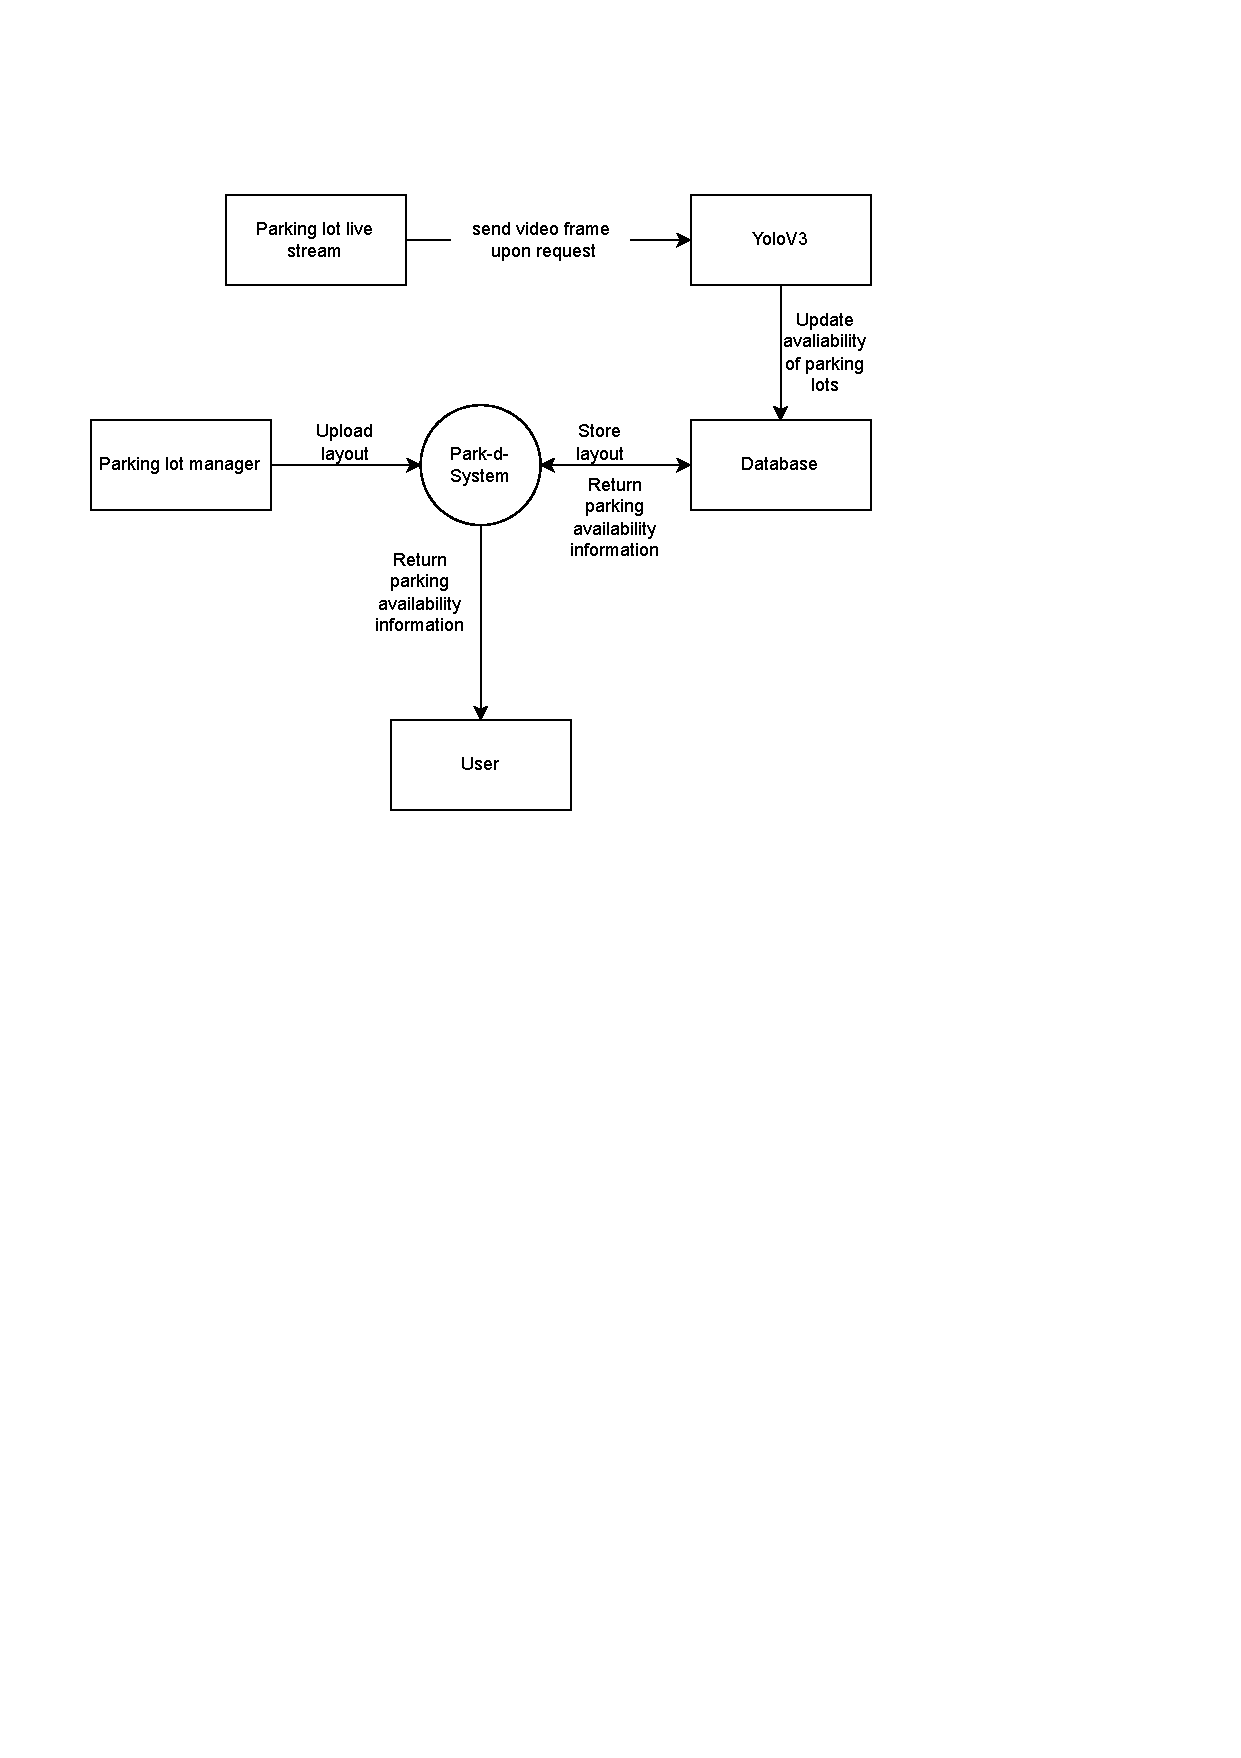
\includegraphics[scale=1.0]{Context_diagram.pdf}
    \end{center}
\end{figure}

\newpage
\clearpage
\subsubsection{Work Partitioning}
\begin{table}[h!]
\caption{Work Partitioning Events}
    \centering
    \begin{tabular}{|c|p{3.5cm}|c|p{3.5cm}|}
    \hline
    \textbf{Event Number} & \centering\textbf{Event Name} & \textbf{Input} &
    \textbf{Output} \\
    \hline
    1 & System start & User data & Parking lot map\\
    \hline
    2 & Find an open spot & Parking lot data & Available spot list\\
    \hline
    3 & Filter spots & Filter specification & Available spot list\\
    \hline
    4 & Valid spot selection & Spot selection & Spot traversal directions\\
    \hline
    5 & Invalid spot selection & Spot selection & Invalid selection\\
    \hline
    6 & Spot traversal & None & Available spot list\\
    \hline
    7 & Traversal complete & Spot reached & System feedback\\
    \hline
    8 & Settings change & Settings list & None\\
    \hline
    9 & Traversal termination & Termination selection & Parking lot map\\
    \hline
    10 & Lot status & Parking lot data & Parking lot stats\\
    \hline
    11 & Layout edit & Parking lot Layout & None\\
    \hline
    \end{tabular}
\end{table}

\begin{table}[h]
\caption{Work Partitioning Summaries}
    \centering
    \begin{tabular}{|c|p{10cm}|}
    \hline
    \textbf{Event Number} & \textbf{Summary} \\
    \hline
    1 & Starting the system. Location data is needed to determine which parking
    lot data to use and where the user is in the parking lot.\\
    \hline
    2 & Use cameras in the parking lot and an AI to recognize open/special
    spots. List these spots to the user.\\
    \hline
    3 & \textcolor{red}{Use special spots such as accessible and reserved
    types.}\\ %Toggle seeing special spots in the list of available spots.\\
    \hline
    4 & Choose a spot in the list of available spots and get directions to it.\\
    \hline
    5 & Choose a spot not on the list of available spots or was filtered out.
    Inform the user to make an appropriate selection.\\
    \hline
    6 & The user follows the directions to the spot. If the status of the spot
    changes, the user will be prompted to change spots.\\
    \hline
    7 & The user reaches the spot. The system data is updated and the user is
    asked for feedback.\\
    \hline
    8 & Adjust system settings like sound, and vehicle details\\
    \hline
    9 & Quit traversing to the current spot and return to the map.\\
    \hline
    \textcolor{red}{10} & \textcolor{red}{View/create/modify parking lots}.\\
    \hline
    11 & Collect statistical data about the parking lot from cameras over time.
    The owner can use this data to make business decisions.\\
    \hline
    12 & Allows the owner to add/remove/modify spots in the layout.\\
    \hline
    \end{tabular}
\end{table}

\newpage

\subsubsection{\textcolor{red}{Individual Product Use Cases}}
\begin{figure}[H]
    \centering
    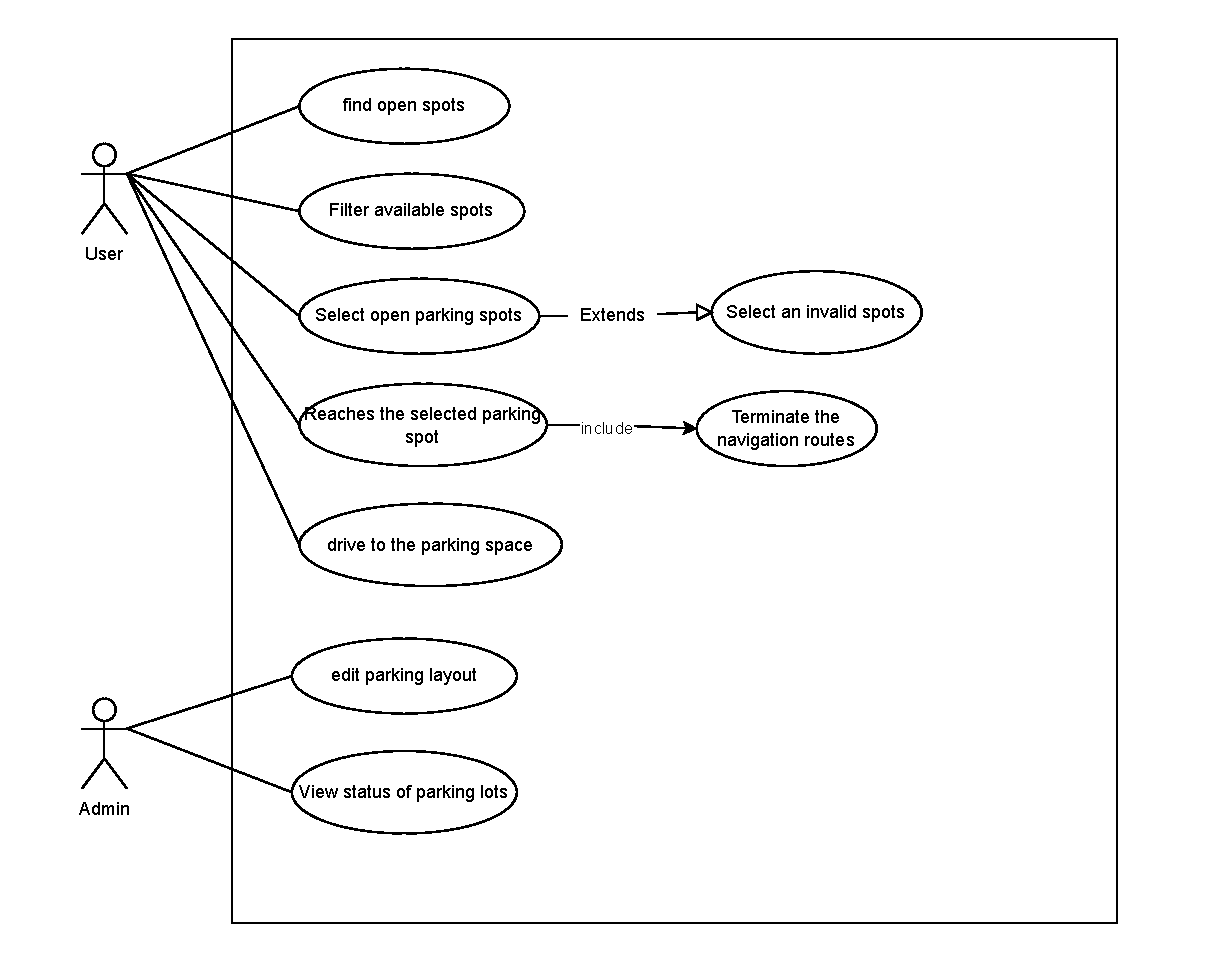
\includegraphics[width=13cm, height=13cm]{use_case.pdf}
    \caption{Use case diagram that displays the main functionalities of the application.}
\end{figure}

\subsection{Functional Requirements}
\refstepcounter{businesseventnum}
\begin{enumerate}[{BE}\thebusinesseventnum.] 
\item The driver wishes to start the system.
\refstepcounter{funcreqnum}
\begin{enumerate}[{FR}\thefuncreqnum.] 
    \item The system must prompt the driver to turn on the driver's location
    data.\\
    \textbf{Rationale:} Location data is required to navigate the driver from
    their current position to their desired parking space in the parking lot.
\end{enumerate}
\refstepcounter{funcreqnum}
\begin{enumerate}[{FR}\thefuncreqnum.] 
    \item The system must present the driver with a map of their surroundings,
    \textcolor{red}{if they have allowed location access}.\\
    \textbf{Rationale:} Upon start-up, the system presenting the map of the
    driver's surroundings will help the driver orient themselves in their
    current location.
\end{enumerate}
\color{red}{
\refstepcounter{funcreqnum}
\begin{enumerate}[{FR}\thefuncreqnum.] 
    \item The system shall disable the navigation component if the driver
    doesn't provide permission.\\
    \textbf{Rationale:} Not all drivers wish to provide permission or use the
    navigation component.
\end{enumerate}
}
\end{enumerate}

\refstepcounter{businesseventnum}
\begin{enumerate}[{BE}\thebusinesseventnum.] 
\item The driver wishes to find an open parking spot.
\refstepcounter{funcreqnum}
\begin{enumerate}[{FR}\thefuncreqnum.] 
    \item The system shall use parking lot camera footage and sensors to survey
    the parking lot. \label{poc1}\\
    \textbf{Rationale:} To determine available spaces in the parking lot, camera
    footage of the parking lot and sensor information need to be collected for
    the parking spaces.
\end{enumerate}
\refstepcounter{funcreqnum}
\begin{enumerate}[{FR}\thefuncreqnum.] 
    \item The system shall \textcolor{red}{allow admins to mark special parking
    spots.}\\ %recognize special parking spots.
    \textbf{Formal Specification: } \[\forall SP | SP \in P  \bullet Detect(SP)
    = true\]\\
    \textcolor{red}{Where SP: special spot, P: parking spot}\\
    \textbf{Rationale:} The system needs to know about these spots so that they
    \textcolor{red}{are only selected by those who need them}.%appear to only
    those who need them.
\end{enumerate}
\refstepcounter{funcreqnum}
\begin{enumerate}[{FR}\thefuncreqnum.] 
    \item The system shall \textcolor{red}{allow admins to mark the physical
    location of parking spots}. \label{poc2}\\ %determine the physical location
    of parking spots. \textbf{Rationale:} Drivers will be directed to their
    spot, so their destination has to be determined by the camera location.
\end{enumerate}
\refstepcounter{funcreqnum}
\begin{enumerate}[{FR}\thefuncreqnum.] 
    \item The system must \color{red}{display all available parking lots and
    allow} the driver to provide the parking lot that they wish to navigate
    to.\\
    \textbf{Formal Specification: }  \\Available spot = \[\forall S | S \in A
    \bullet x < x1 \land  x < x3 \land x > x2 \land x > x4 \land y < y1 \land  y
    < y3 \land y > y2 \land y > y4 = true\]\\
    Where T = (x,y) be a pair of coordinates indicates the mid point of the
    detected vehicle.\\
    S = [(x1,y1), (x2,y2), (x3,y3), (x4,y4)] be an array of 4 tuples with each
    tuple represent the coordinates of a parking space annotation from top left
    corner to bottom right corner in counter-clock wise direction\\
    And A be a set of S\\
   
\end{enumerate}
\refstepcounter{funcreqnum}
\begin{enumerate}[{FR}\thefuncreqnum.] 
    \item The system must display the available parking spaces of the specified
    destination parking lot.
\end{enumerate}
\end{enumerate}

\refstepcounter{businesseventnum}
\begin{enumerate}[{BE}\thebusinesseventnum.] 
\item The driver wishes to filter the available parking spots.
\refstepcounter{funcreqnum}
\begin{enumerate}[{FR}\thefuncreqnum.] 
    \item The system shall allow the driver to select between using available
    normal, accessibility and reserved parking spaces, \textcolor{red}{with
    confirmation of authorization for the latter two}.\\
    \textbf{Rationale:} The driver should be able to view and select between all
    possible types of parking spaces if they are authorized. For example, a
    driver with a wheelchair would need to see accessible parking spaces,
    whereas, an able-bodied driver would only need to use normal parking spaces
    to avoid parking in an accessible or reserved parking space.
\end{enumerate}
\refstepcounter{funcreqnum}
\begin{enumerate}[{FR}\thefuncreqnum.] 
    \item The system by default must \textcolor{red}{only allow selections for
    normal, non-reserved parking spaces, if authorization is not
    confirmed.}\\%display only normal, non-reserved parking spaces.\\
    \textbf{Rationale:} Most drivers will not be authorized to use accessible
    parking spaces or reserved parking spaces, such as those for public transit
    vehicles. Without any other input, the system should allow only the spaces
    that the most drivers can use.
\end{enumerate}
\end{enumerate}

\refstepcounter{businesseventnum}
\begin{enumerate}[{BE}\thebusinesseventnum.] 
\item The driver wishes to select an open parking spot.
\refstepcounter{funcreqnum}
\begin{enumerate}[{FR}\thefuncreqnum.] 
    \item The system shall allow the driver to select an available parking
    space.\\
    \textbf{Rationale:} The driver must be allowed to select an available
    parking space to receive instructions to park at the desired parking space.
\end{enumerate}

\refstepcounter{funcreqnum}
\begin{enumerate}[{FR}\thefuncreqnum.] 
    \item The system shall display driving directions to the driver upon
    selecting an available parking space.\\
    \textbf{Rationale:} The driver should be informed on how to reach the
    parking space they selected from their current position.
\end{enumerate}

\color{red}{
\refstepcounter{funcreqnum}
    \begin{enumerate}[{FR}\thefuncreqnum.] 
        \item The system shall provide a default recommendation if the driver
        does not wish or is not able to select a specific parking space.
        \label{poc3}\\
        \textbf{Rationale:} Providing the input to select a specific parking
        space may be difficult on small displays because of the relative size
        difference between a parking lot and a space.\\
        \textbf{Will be implemented in a future revision.}
    \end{enumerate}
}

\color{red}{
\refstepcounter{funcreqnum}
\begin{enumerate}[{FR}\thefuncreqnum.] 
    \item The system shall display navigation directions to the default
    recommended parking space if the driver makes no space selection within
    $\hyperlink{default_delay}{DEFAULT\_DELAY}$ seconds.\\
    \textbf{Will be implemented in a future revision.}
\end{enumerate}
}

\end{enumerate}

\refstepcounter{businesseventnum}
\begin{enumerate}[{BE}\thebusinesseventnum.] 
\item The driver wishes to select an invalid parking spot.

    \refstepcounter{funcreqnum}
    \begin{enumerate}[{FR}\thefuncreqnum.] 
    \color{red}
        \item The system shall not allow the driver to select an invalid spot
        such as spots that are already occupied.\\
        \textbf{Rationale:} The driver should not be able to select an invalid
        spot.
    \end{enumerate}

\refstepcounter{funcreqnum}
\begin{enumerate}[{FR}\thefuncreqnum.] 
    \item The system shall notify the driver if they attempt to select a
    reserved or disabled parking space, if they have confirmed authorization for
    those spaces.\\
    \textbf{Rationale:} The driver should be informed that they cannot park in a
    spot that requires other authorization.
\end{enumerate}

\end{enumerate}

\refstepcounter{businesseventnum}
\begin{enumerate}[{BE}\thebusinesseventnum.] 
\item The driver wishes to drive to the parking space.
\refstepcounter{funcreqnum}
\begin{enumerate}[{FR}\thefuncreqnum.] 
    \item The system shall provide real time directions to the driver to the
    selected parking space.
\end{enumerate}

\color{red}{
\refstepcounter{funcreqnum}
    \begin{enumerate}[{FR}\thefuncreqnum.] 
        \item The system shall recommend a new available parking space to the
        driver upon the initial selected parking space being taken.\\
        \textbf{Will be implemented in a future revision.}
    \end{enumerate}
}

\color{red}{
\refstepcounter{funcreqnum}
\begin{enumerate}[{FR}\thefuncreqnum.] 
    \item The system shall provide the option to safely select a new parking
    space upon the initial selected parking space being taken.\\
    \textbf{Will be implemented in a future revision.}
\end{enumerate}
}

\color{red}{
\refstepcounter{funcreqnum}
\begin{enumerate}[{FR}\thefuncreqnum.] 
    \item The system shall terminate the route and inform the driver if the
    chosen space has been taken before they arrive.\\
    \textbf{Rationale:} The driver must choose a new space when theirs is taken.
\end{enumerate}
}

\color{red}{
\refstepcounter{funcreqnum}
\begin{enumerate}[{FR}\thefuncreqnum.] 
    \item The system shall terminate the route if the driver doesn't arrive
    within a time estimate plus
    $\hyperlink{timeout_tolerance}{TIMEOUT\_TOLERANCE}$ seconds.\\
    \textbf{Formal Specification: }
    \[\texttt{T} \geq \texttt{TimeOutTolerance} \Rightarrow Ter\] \\
    \[\texttt{T} \leq \texttt{TimeOutTolerance} \Rightarrow Wor\] 
    
    Where TimeOutTolerance: the maximum time that system do not terminate when
    user's hasn't arrive to the Destination\\
    Where Ter is the termination state\\
    Where Wor is the working state\\
    Where T is the time has elapsed after user start navigation\\
    \textbf{Rationale:} The driver may take too long to reach the space or not
    go at all.
\end{enumerate}
}

\color{red}{
\refstepcounter{funcreqnum}
\begin{enumerate}[{FR}\thefuncreqnum.] 
    \item The system shall track the driver's location within
    $\hyperlink{distance_tolerance}{DISTANCE\_TOLERANCE}$ meters.\\
    \textbf{Rationale:} Location data isn't perfect so there must be a
    tolerance.
\end{enumerate}
}

\color{red}{
\refstepcounter{funcreqnum}
\begin{enumerate}[{FR}\thefuncreqnum.] 
    \item The system shall provide a time estimate to the selected space within
    $\hyperlink{driving_estimate_tolerance}{DRIVING\_ESTIMATE\_TOLERANCE}$
    seconds.\\
    \textbf{Rationale:} Drivers should take driving time in to consideration
    when finding a spot.
\end{enumerate}
}

\end{enumerate}

\refstepcounter{businesseventnum}
\begin{enumerate}[{BE}\thebusinesseventnum.] 
\item The driver reaches the selected parking spot.
\refstepcounter{funcreqnum}
\begin{enumerate}[{FR}\thefuncreqnum.] 
    \item The system shall prompt the driver that they have reached the parking
    spot. \label{poc4}
\end{enumerate}

\refstepcounter{funcreqnum}
\begin{enumerate}[{FR}\thefuncreqnum.] 
    \item The system shall change the status of the parking space from available
    to unavailable when the driver enters the parking space. \label{poc5}\\
    \textbf{Rationale:} Using the driver's location within the parking lot, the
    status of the parking space should be updated, such that future drivers do
    not pick the same parking space.
\end{enumerate}
\color{red} {
\refstepcounter{funcreqnum}
\begin{enumerate}[{FR}\thefuncreqnum.] 
    \item The system shall non-intrusively prompt the driver for feedback
    regarding their experience after parking.\\
    \textbf{Rationale:} Driver feedback will be important to improve our
    system's experience, as well as to alert us of any issues they have
    encountered.\\
    \textbf{Will be implemented in a future revision.}
\end{enumerate}
}
\end{enumerate}

\refstepcounter{businesseventnum}
\begin{enumerate}[{BE}\thebusinesseventnum.] 
\color{red} {
\item The driver wishes to change the settings of the application. } \color{red}
{
\refstepcounter{funcreqnum}
\begin{enumerate}[{FR}\thefuncreqnum.] 
    \item The system shall provide a means of viewing and modifying the
    settings.\\
    \textbf{Will be implemented in a future revision.}
\end{enumerate}
} \color{red} {
\refstepcounter{funcreqnum}
\begin{enumerate}[{FR}\thefuncreqnum.] 
    \item The system's settings menu shall include volume and sound adjustment,
    unit identification, vehicle details, and notification preferences.\\
    \textbf{Will be implemented in a future revision.}
\end{enumerate}
}
\end{enumerate}

\refstepcounter{businesseventnum}
\begin{enumerate}[{BE}\thebusinesseventnum.] 
\item The driver wishes to terminate the current navigation route.
\refstepcounter{funcreqnum}
\begin{enumerate}[{FR}\thefuncreqnum.] 
    \item The system shall provide a means to terminate the current navigation.
\end{enumerate}
\refstepcounter{funcreqnum}
\begin{enumerate}[{FR}\thefuncreqnum.] 
    \item The system shall present the driver in their current location on the
    map upon termination of the route.
\end{enumerate}
\end{enumerate}

\refstepcounter{businesseventnum}
\begin{enumerate}[{BE}\thebusinesseventnum.] 
\item The parking lot owner/manager wishes to view the current status of their
parking lot.
\refstepcounter{funcreqnum}
\begin{enumerate}[{FR}\thefuncreqnum.] 
    \item The system must provide a separate administrative view for parking lot
    owners/managers.
\end{enumerate}
\refstepcounter{funcreqnum}
\begin{enumerate}[{FR}\thefuncreqnum.] 
    \item The system must provide a means for individual parking lot
    owners/managers to enter their own administrative console.
\end{enumerate}
\refstepcounter{funcreqnum}
\begin{enumerate}[{FR}\thefuncreqnum.] 
    \item The system's administrative console shall provide a means for the
    parking lot owner/manager to view the availability of all parking spaces in
    their lot.
\end{enumerate}
\end{enumerate}

\color{red} {
    \refstepcounter{businesseventnum}
    \begin{enumerate}[{BE}\thebusinesseventnum.] 
    \item The parking lot owner/manager or driver wishes to view the analytics
    of their desired parking lot.
    
    \refstepcounter{funcreqnum}
    \begin{enumerate}[{FR}\thefuncreqnum.] 
        \item The system shall display live analytics on how many spaces are
        available/unavailable and categorize them in terms of their type
        (standard, accessible, reserved).
    \end{enumerate}

    \refstepcounter{funcreqnum}
    \begin{enumerate}[{FR}\thefuncreqnum.] 
        \item The system shall display twenty-four hours of averaged historical
        parking lot occupancy information.
    \end{enumerate}
    \end{enumerate}
}

\color{black}
\refstepcounter{businesseventnum}
\begin{enumerate}[{BE}\thebusinesseventnum.] 
\item The parking lot owner/manager wishes to edit their parking lot layout.
\refstepcounter{funcreqnum}
\begin{enumerate}[{FR}\thefuncreqnum.] 
    \item The system's administrative console shall include a means for
    individual parking lot owners/managers to edit their parking lot layout.
\end{enumerate}
\refstepcounter{funcreqnum}
\begin{enumerate}[{FR}\thefuncreqnum.] 
    \item The system's administrative console shall include editing features
    such as redefining parking spaces and marking spaces as reserved.
\end{enumerate}
\end{enumerate}

%%%%%%%%%%%%%%%%%%%%%%%%%%%%%%%%%%%% Non-functional Requirements
%%%%%%%%%%%%%%%%%%%%%%%%%%%%%%%%%%%%%
\section{Non-functional Requirements}
This section specifies the non-functional requirements for Park'd.
\subsection{Look and Feel Requirements}
\subsubsection{Appearance Requirements}
\begin{enumerate}[{LF}1.] 
    \item The user interface must only consist of information immediately
    relevant to the driver. \label{pocnf1} \\
    \textbf{Fit Criterion:} For every element of the interface, all
    \textbf{Park'd} developers agree on its necessity.
\end{enumerate}

\color{red}
\subsubsection{Style Requirements}
\begin{enumerate}[resume*]  
    \item All user interface elements must conform to the park-d branding
    guidelines\\
    \textbf{Fit Criterion:} All the user interface elements presented in our
    website should have consistent use of the organization's logo, font, and
    yellow black color scheme.
\end{enumerate}

\color{black}
\subsection{Usability and Humanity Requirements}
\subsubsection{Ease of Use Requirements}
\begin{enumerate}[{UH}1.] 
    \item Operations from the working screen take no more than
    $\hyperlink{max_taps}{MAX\_TAPS}$ taps to complete.\\
    \color{red}
    \item For each function feature in the software, novice users are able to
    identify and complete each of them with no more than
    $\hyperlink{max_time_complete}{MAX\_COMPLETE\_TIME}$ minute \\
\end{enumerate}
\color{black}

\subsubsection{Personalization and Internationalization Requirements}
\noindent \emph{N/A}

\subsubsection{Learning Requirements}
\begin{enumerate}[resume*] 
    \item The system's basic parking functionality should be useable with no
    prior instruction. \label{pocnf2}\\
    \textbf{Fit Criterion:} 80\% of testers navigate to a designated parking
    spot without any prior instruction. 
\end{enumerate}

\subsubsection{Understandability and Politeness Requirements}
\begin{enumerate}[resume*] 
    \item Any symbols must be understandable to the driver. \label{pocnf3} \\
    \textbf{Fit Criterion:} All symbols used adhere to the standard set forth by
    the Ontario Ministry of Transportation.
\end{enumerate}

\subsubsection{Accessibility Requirements}
\noindent \emph{N/A}

\subsection{Performance Requirements}
\subsubsection{Speed and Latency Requirements}
\begin{enumerate}[{PE}1.] 
\color{red}{
    \item The system must maintain a minimum of
    $\hyperlink{min_framerate}{MIN\_FRAMERATE}$ during normal operation.\\
}
\end{enumerate}

\subsubsection{Safety-Critical Requirements}
\begin{enumerate}[resume*] 
    \item The system must never direct driver user off of the road, for example,
    onto the sidewalk.\\
    \textbf{Fit Criterion:} Computer constructed maps of the parking lot will be
    inspected by the developers to ensure no deviations from the marked
    surfaces.
    \item The system must never direct the user to park in a reserved area such
    as a fire lane or across a driveway.\\
    \textbf{Fit Criterion:} Computer constructed maps of the parking lot will be
    inspected by the developers to ensure only marked parking spots are
    recognized.
\end{enumerate}

\subsubsection{Precision or Accuracy Requirements}
\noindent \emph{N/A}

\subsubsection{Reliability and Availability Requirements}
\color{red}{
\begin{enumerate}[resume*] 
    \item The system shall be responsive, that is, it should respond to the
    user's command within $\hyperlink{default_delay}{DEFAULT\_DELAY}$/4
    seconds.\\
    \textbf{Fit Criterion:} We require for the maximum delay to be
    $\hyperlink{default_delay}{DEFAULT\_DELAY}$/4 because, based on user
    validation testing, users began to voice their frustration after
    $\hyperlink{default_delay}{DEFAULT\_DELAY}$/4 seconds. 
\end{enumerate}
}
\color{black}


\subsubsection{Robustness or Fault-Tolerance Requirements}
\begin{enumerate}[resume*] 
\color{red}{
    \item In the event of lost connection to the system back-end, the most
    recent recommended parking spot will remain on the display.\\
    }
\end{enumerate}

\subsubsection{Capacity Requirements}
\begin{enumerate}[resume*] 
\color{red}{
    \item The system back-end must support
    $\hyperlink{concurrent_users}{CONCURRENT\_USERS}$ using the system at the
    same time.\\
    }
\end{enumerate}

\subsubsection{Scalability or Extensibility Requirements}
\begin{enumerate}[resume*] 
    \color{red}{\item The system shall provide administrators the ability to add
    any number of parking areas ($\hyperlink{parking_lots}{PARKING\_LOTS}$ and
    above) without having to remove previous parking areas.\\}
    \color{black}
\end{enumerate}

\subsubsection{Longevity Requirements}
\noindent \emph{N/A}

\subsection{Operational and Environmental Requirements}
\subsubsection{Expected Physical Environment}
\begin{enumerate}[{OE}1.] 
    \item The system shall be operated by a driver in a vehicle. \label{pocnf4}
    \\
    \textbf{Fit Criterion:} The system is designed for a vehicle app or a device
    to travel with.
\end{enumerate}

\subsubsection{Requirements for Interfacing with Adjacent Systems}
\noindent \emph{N/A}

\subsubsection{Productization Requirements}
\noindent \emph{N/A}

\subsubsection{Release Requirements}
\begin{enumerate}[resume*] 
    \item The system shall have a new release at least once a month as GitHub
    commits.\\
    \textbf{Fit Criterion:} Check GitHub commit log for update frequency.
\end{enumerate}

\subsection{Maintainability and Support Requirements}
\subsubsection{Maintenance Requirements}
\color{red}
\begin{enumerate}[{MA}1.] 
    \item Critical issues will be addressed immediately with a target resolution
    time. Issues will be tracked and prioritized based on severity and impact on
    system functionality. \\
    \textbf{Fit Criterion:} The software issues and bugs should be resolved in
    less than 24 hours after errors or bugs being located. A dedicated team
    member will be responsible for identifying, prioritizing, and addressing
    maintenance issues and these issues will be recorded with their severity in
    a internal document.
\end{enumerate}
\color{black}

\subsubsection{Supportability Requirements}
\begin{enumerate}[resume*] 
    \item The system shall provide drivers with instructions and contacts in the
    interface.\\
    \textbf{Fit Criterion:} At least
    $\hyperlink{supportability_satisfaction}{SUPPORTABILITY\_SATISFACTION}$ of
    surveyed drivers are satisfied with their support.
\end{enumerate}

\subsubsection{Adaptability Requirements}
\noindent \emph{N/A}

\subsection{Security Requirements}
\subsubsection{Access Requirements}
\begin{enumerate}[{SR}1.] 
    \item The system's parking lot data shall be accessible only to the team and
    to the property owner(s).\label{pocnf5} \\
    \textbf{Fit Criterion:} The data is password protected.
    \item Only the parking lot owner(s) shall have the option to edit the
    parking space layout \label{asr2} \\
    \color{red}{\textbf{Fit Criterion:} Upon logging in as a standard user,
    there should not be a button to edit the layout of any parking area. For an
    administrator, there should only be a button to edit the layout of the
    parking lot that they own.}
    \color{black}
    \item Only the parking space manager(s) of a parking lot are allowed to have
    access to the administrative console for their parking lot \label{asr3}\\
    \textbf{Fit Criterion:} The administrative console of a parking lot can only
    edit and view analytics of the parking lot
\end{enumerate}

\subsubsection{Integrity Requirements}
\begin{enumerate}[resume*] 
    \item The system shall prevent inaccurate data from being stored.\\
    \textbf{Fit Criterion:} Stress test the system with accurate and inaccurate
    data and measure the data's accuracy.\\
    \textbf{\textcolor{red}{Will be implemented in a future revision.}}
    \item Unsaved parking layout information should be stored locally if the
    information cannot be uploaded to the server \label{isr5}\\
    \textbf{\textcolor{red}{Will be implemented in a future revision.}}
    \item{\color{red} Unsaved parking layout information should attempt to
    upload to the server every
    $\hyperlink{attempt_upload_time}{ATTEMPT\_UPLOAD\_TIME}$ seconds
    \label{isr6}\\
    \textbf{Will be implemented in a future revision.}}
    \item{\color{red}Parking layouts will be automatically backed up daily
    \label{isr7}\\
    \textbf{Will be implemented in a future revision.}}
    \item No parking space should be stored in a different format in the
    database from other parking spaces \label{isr8}
    \item The system should only allow a parking spot to have
    $\hyperlink{max_special_property}{MAXIMUM\_SPECIAL\_PROPERTY}$ special
    property \label{isr9}\\
    \textbf{Fit Criterion:} A parking space is either labeled as accessibility,
    electric vehicle, or reserved
    \item Parking lot managers must be prompted when there is a failed attempt
    to add a parking spot to the database \label{isr10}
    \item Parking lot owners should be able to prompt the upload of their
    parking lot layout to the database and server \label{isr11}
    \item Correct paths should be stored to all parking spaces \label{isr12}
    \item Users are informed when an error occurs when the system is determining
    the navigation path \label{isr13}
\end{enumerate}

\subsubsection{Privacy Requirements}
\begin{enumerate}[resume*] 
    \item The system shall ask for permission to use the driver's location
    data.\\
    \textbf{Fit Criterion:} The system has a driver location agreement form.
\end{enumerate}

\subsubsection{Audit Requirements}
\noindent \emph{N/A}

\subsubsection{Immunity Requirements}
\noindent \emph{N/A}

\subsection{Cultural and Political Requirements}
\subsubsection{Cultural Requirements}
\noindent \emph{N/A}

\subsubsection{Political Requirements}
\noindent \emph{N/A}

\subsection{Legal Requirements}
\subsubsection{Compliance Requirements}
\begin{enumerate}[{LR}1.] 
    \item The system shall follow laws relating to device usage while driving.\\
    \textbf{Fit Criterion:} The laws relating to device usage while driving
    should be referenced and checked for compliance.
\end{enumerate}
\subsubsection{Standards Requirements}
\noindent \emph{N/A}

\subsection{Health and Safety Requirements}
\begin{enumerate}[{HS}1.] 
    \item The system shall not include flashing graphics or disturbing
    imagery.\\
    \textbf{Fit Criterion:} Drivers surveyed should not find the system
    distracting or disturbing.
\end{enumerate}

\newpage
\section{Priority Requirements}
\label{priorityreqs}
High priority requirements are identified here, as well as requirements that are
unlikely to change.

\subsection{Requirements for the Proof of Concept}
\textbf{November 7:} The following requirements will need to be met at least one
week before the proof of concept demonstrations begin, from November 14-25. The
proof of concept plan can be found within the
\href{https://github.com/parkd-app/park-d/blob/main/docs/DevelopmentPlan/DevelopmentPlan.pdf}
{Development Plan}. This is to allow time for debugging and polish. These
requirements are fundamental to the basic function of the system.
\begin{itemize}
    \item \hyperref[poc1]{BE2FR4}: The system must have access to useable
    parking area footage.
    \item \hyperref[poc2]{BE2FR6}: The system must be able to process footage to
    construct a valid parking space.
    \item \hyperref[poc3]{BE4FR13}: The system will be demonstrated with a
    single parking space.
    \item \hyperref[poc4]{BE7FR24}: The system must recognize and relay to the
    driver when they have arrived to the space.
    \item \hyperref[poc5]{BE7FR25}: The system must mark the space as full once
    a vehicle has entered it.
    \item \hyperref[pocnf1]{LF1}: The user interface should not need to be
    simplified over time.
    \item \hyperref[pocnf2]{UH3}: With only basic functionality, minimal
    instruction should be needed.
    \item \hyperref[pocnf3]{UH4}: We should not introduce any symbols that would
    be unfamiliar to the driver.
    \item \hyperref[pocnf4]{OE1}: The system will be developed for drivers.
    \item \hyperref[pocnf5]{SR1}: The video feed should never be accessible from
    the front-end, because it is processed by the back-end.
\end{itemize}

\subsection{Requirements for Full Revisions}
\textbf{January 31:} All other requirements set out in this document are to be
met two weeks before the Revision 0 demonstration, which will occur between
February 6-17. The additional margin is because extensive debugging and testing
will likely be needed at this stage. At this time, the team will also begin to
consider the addition of further requirements to meet our stretch goals.

\textbf{March 13:} Revision 1 will likely include the addition of some stretch
goals, for which requirements will be added to this document. Those requirements
will need to be fulfilled at least one week prior to the Revision 1
demonstrations, on March 20-31.

\subsection{Requirements Unlikely to Change}
\textcolor{red}{\st{Non-functional requirements relating to the user experience
are unlikely to change because they do not rely on any specific software or
hardware limitations. Instead, they specify how we will make some design
decisions on the front-end to benefit drivers and administrators. }}

\textcolor{red}{\st{Requirements relating to the law such as parking in disabled
parking spaces are unlikely to change because these laws are well established
and unlikely to change. It would be irresponsible to release an application that
recommends breaking the law and risking a ticket or a tow.}}

\textcolor{red}{All requirements except for FR20, FR26, AND MA1 are unlikely to
change.\\
FR20: The system might be changed to automatically redirect the user to another
spot if it is close enough to the original spot selected.\\
FR26: Rather than prompting the user for feedback, the system may include
another method for users voluntarily offer feedback as it may become annoying
for the users to get a prompt after every session.\\
MA1: As the system scales and expands in the future, the maintenance procedure
may have to change to support more features and users.}


\newpage
\section{Traceability Between Functional and Non-Functional Requirements}
Traceability between functional and non-functional requirements is shown by a
series of traceability matrices mapping functional requirements to
non-functional requirements.
\label{traceabilityMatrixSection}
\subsection{Traceability Between Test Cases and Requirements}
\begin{landscape}
\begin{table}[htbp]
\caption{Traceability Matrix for Functional and Non-Functional Requirements -
Part 1} \label{traceMatrix1} \scalebox{0.8}{
\begin{tabularx}{\textwidth}{cc|c|c|c|c|c|c|c|c|c|c|c|c|c|c|}
\cline{3-16}
& & \multicolumn{14}{ c|}{Non-Functional Requirements} \\ \cline{3-16} & & LF1 &
LF2 & UH1 & UH2 & UH3 & UH4 & PE1 & PE2 & PE3 & PE4 & PE5 & PE6 & OE1 & OE2 \\
\cline{1-16} \multicolumn{1}{ |c| }{\multirow{31}{*}{Functional Requirements} }
& \multicolumn{1}{|c| } {FR1}   &X&X&X&X& &X&X&X&X& &X& &X& \\ \cline{2-16}
\multicolumn{1}{|c| }{} 	                  & \multicolumn{1}{|c| }{FR2}
&X&X&X&X& &X&X&X&X& & & &X& \\ \cline{2-16} \multicolumn{1}{|c| }{} &
\multicolumn{1}{|c| } {FR3}   & & & & & & & &X&X& & & & & \\ \cline{2-16}
\multicolumn{1}{|c| }{}                        & \multicolumn{1}{ |c| } {FR4}  &
& & & & & & & & &X& & & & \\ \cline{2-16} \multicolumn{1}{|c| }{} &
\multicolumn{1}{ |c| } {FR5}  & & & & & & & &X&X&X& & & & \\ \cline{2-16}
\multicolumn{1}{|c| }{}                        & \multicolumn{1}{ |c| } {FR6}
&X&X&X&X&X&X&X& & & & & &X& \\ \cline{2-16} \multicolumn{1}{|c| }{} &
\multicolumn{1}{ |c| } {FR7}  &X&X& &X&X&X&X&X&X&X& & & & \\ \cline{2-16}
\multicolumn{1}{|c| }{}                        & \multicolumn{1}{ |c| } {FR8}
&X&X&X&X&X&X&X& & & & & &X& \\ \cline{2-16} \multicolumn{1}{|c| }{} &
\multicolumn{1}{ |c| } {FR9}  & & & & &X& &X& & & & & & & \\ \cline{2-16}
\multicolumn{1}{|c| }{}                        & \multicolumn{1}{ |c| } {FR10} &
& & & &X& &X&X&X&X& & &X& \\ \cline{2-16} \multicolumn{1}{|c| }{} &
\multicolumn{1}{ |c| } {FR11} &X&X& &X&X&X&X&X&X&X& & &X& \\ \cline{2-16}
\multicolumn{1}{|c| }{}                        & \multicolumn{1}{ |c| } {FR12} &
& & & & & &X&X&X&X& & &X& \\ \cline{2-16} \multicolumn{1}{|c| }{} &
\multicolumn{1}{ |c| } {FR13} & & & & &X& &X&X&X&X& & &X& \\ \cline{2-16}
\multicolumn{1}{|c| }{}                        & \multicolumn{1}{ |c| } {FR14}
&X&X& &X& &X&X&X&X& & & &X& \\ \cline{2-16} \multicolumn{1}{|c| }{} &
\multicolumn{1}{ |c| } {FR15} &X&X& &X& &X&X&X&X& & & &X& \\ \cline{2-16}
\multicolumn{1}{|c| }{}                        & \multicolumn{1}{ |c| } {FR16} &
& & & &X& &X&X&X&X&X& &X& \\ \cline{2-16} \multicolumn{1}{|c| }{} &
\multicolumn{1}{ |c| } {FR17} & & & & &X& &X&X&X& & & &X& \\ \cline{2-16}
\multicolumn{1}{|c| }{}                        & \multicolumn{1}{ |c| } {FR18}
&X&X& &X&X&X&X&X&X&X& & &X& \\ \cline{2-16} \multicolumn{1}{|c| }{} &
\multicolumn{1}{ |c| } {FR19} &X&X& &X&X&X&X&X&X& & & &X& \\ \cline{2-16}
\multicolumn{1}{|c| }{}                        & \multicolumn{1}{ |c| } {FR20} &
& & & & & &X& & & & & & & \\ \cline{2-16} \multicolumn{1}{|c| }{} &   
\multicolumn{1}{ |c| } {FR21} &X&X& &X&X&X&X& & & & & &X& \\ \cline{2-16}
\multicolumn{1}{|c| }{}                        &   
\multicolumn{1}{ |c| } {FR22} &X&X& &X& &X&X& & & & & &X& \\ \cline{2-16}
\multicolumn{1}{|c| }{}                        &   
\multicolumn{1}{ |c| } {FR23} &X&X& &X& &X&X& & & & & &X& \\ \cline{2-16}
\multicolumn{1}{|c| }{}                        &   
\multicolumn{1}{ |c| } {FR24} & & & & &X& &X& & & & & &X& \\ \cline{2-16}
\multicolumn{1}{|c| }{}                        &   
\multicolumn{1}{ |c| } {FR25} &X&X& &X&X&X&X& & & & & &X& \\ \cline{2-16}
\multicolumn{1}{|c| }{}                        &   
\multicolumn{1}{ |c| } {FR26} & & & & & & &X& & & & & & & \\ \cline{2-16}
\multicolumn{1}{|c| }{}                        &   
\multicolumn{1}{ |c| } {FR27} & & & & & & & & & & & & & & \\ \cline{2-16}
\multicolumn{1}{|c| }{}                        &   
\multicolumn{1}{ |c| } {FR28} & & & & & & &X& & & & & & & \\ \cline{2-16}
\multicolumn{1}{|c| }{}                        &   
\multicolumn{1}{ |c| } {FR29} & & & & & & & & & & & & & & \\ \cline{2-16}
\multicolumn{1}{|c| }{}                        &   
\multicolumn{1}{ |c| } {FR30} & & & & & & &X& & & & & & & \\ \cline{2-16}
\multicolumn{1}{|c| }{}                        &   
\multicolumn{1}{ |c| } {FR31} & & & & & & &X& & & & & & & \\ \cline{2-16}
\multicolumn{1}{|c| }{}                        &    
\multicolumn{1}{ |c| } {FR32} & &X&X&X& & &X& & & & & &X& \\ \cline{2-16}
\multicolumn{1}{|c| }{}                        &   
\multicolumn{1}{ |c| } {FR33} & & &X&X& & &X&X&X& & & & & \\ \cline{2-16}
\multicolumn{1}{|c| }{}                        &   
\multicolumn{1}{ |c| } {FR34} & &X& & & & &X& & & & & & & \\ \cline{2-16}
\multicolumn{1}{|c| }{}                        &   
\multicolumn{1}{ |c| } {FR35} & & &X&X& & & &X& & &X& &X& \\ \cline{2-16}
\multicolumn{1}{|c| }{}                        &   
\multicolumn{1}{ |c| } {FR36} & & & & & & &X&X&X& & & &X& \\ \cline{2-16}
\multicolumn{1}{|c| }{}                        &   
\multicolumn{1}{ |c| } {FR37} & & &X&X& & &X& & & & & &X& \\ \cline{1-16}
\end{tabularx}
}
\end{table}
\newpage
\begin{table}[htbp]
\caption{Traceability Matrix for Functional and Non-Functional Requirements -
Part 2} \label{traceMatrix1} \scalebox{0.8}{
\begin{tabularx}{\textwidth}{cc|c|c|c|c|c|c|c|c|c|c|c|c|c|c|}
\cline{3-16}
& & \multicolumn{14}{ c|}{Non-Functional Requirements} \\ \cline{3-16} & & MA1 &
MA2 & SR1 & SR2 & SR3 & SR4 & SR5 & SR6 & SR7 & SR8 & SR9 & SR10 & SR11 & SR12
\\ \cline{1-16} \multicolumn{1}{ |c| }{\multirow{31}{*}{Functional Requirements}
} & \multicolumn{1}{|c| } {FR1}   &&&&&&&&&&&&&& \\ \cline{2-16}
\multicolumn{1}{|c| }{} 	                  & \multicolumn{1}{|c| }{FR2}
&&X&&&&&&&&&&&& \\ \cline{2-16} \multicolumn{1}{|c| }{}                        &
\multicolumn{1}{|c| } {FR3}   &&&X&&&X&&&&X&&&&X \\ \cline{2-16}
\multicolumn{1}{|c| }{}                        & \multicolumn{1}{ |c| } {FR4}
&X&&X&&&X&&&&X&X&&& \\ \cline{2-16} \multicolumn{1}{|c| }{} & \multicolumn{1}{
|c| } {FR5}  &&X&X&&&&&&&&&&&X \\ \cline{2-16} \multicolumn{1}{|c| }{}
& \multicolumn{1}{ |c| } {FR6} &X&&&&&&&&&&&&& \\ \cline{2-16}
\multicolumn{1}{|c| }{}                        & \multicolumn{1}{ |c| } {FR7}
&&&&&&&&&&&&&& \\ \cline{2-16} \multicolumn{1}{|c| }{}                        &
\multicolumn{1}{ |c| } {FR8}  &X&&&&&&&&&&&&& \\
\cline{2-16} \multicolumn{1}{|c| }{}                        & \multicolumn{1}{
|c| } {FR9}  &X&&X&&&&&&&&X&&& \\ \cline{2-16} \multicolumn{1}{|c| }{} &
\multicolumn{1}{ |c| } {FR10} &X&&&&&&&&&&&&& \\ \cline{2-16}
\multicolumn{1}{|c| }{}                        & \multicolumn{1}{ |c| } {FR11}
&X&&&&&&&&&&&&&X \\ \cline{2-16} \multicolumn{1}{|c| }{} & \multicolumn{1}{ |c|
} {FR12} &X&&&&&&&&&&&&& \\ \cline{2-16} \multicolumn{1}{|c| }{}
& \multicolumn{1}{ |c| } {FR13} &X&&&&&&&&&&&&&X \\ \cline{2-16}
\multicolumn{1}{|c| }{} & \multicolumn{1}{ |c| } {FR14} &&&&&&X&&&&&&&& \\
\cline{2-16} \multicolumn{1}{|c| }{}                        & \multicolumn{1}{
|c| } {FR15} &&&&&&X&&&&&&&& \\ \cline{2-16} \multicolumn{1}{|c| }{}
& \multicolumn{1}{ |c| } {FR16} &X&&&&&&&&&&&&&X \\ \cline{2-16}
\multicolumn{1}{|c| }{}                        & \multicolumn{1}{ |c| } {FR17}
&&X&&&&&&&&&&&&\\ \cline{2-16} \multicolumn{1}{|c| }{}                        &
\multicolumn{1}{ |c| } {FR18} &&X&&&&&&&&&&&& \\ \cline{2-16}
\multicolumn{1}{|c| }{}                        & \multicolumn{1}{ |c| } {FR19}
&X&&&&&&&&&&&&& \\ \cline{2-16} \multicolumn{1}{|c| }{}                        &
\multicolumn{1}{ |c| } {FR20} &&&&&&X&&&&&&&& \\ \cline{2-16}
\multicolumn{1}{|c| }{}                        &   
\multicolumn{1}{ |c| } {FR21} &&&&&&&&&&&&&& \\ \cline{2-16} \multicolumn{1}{|c|
}{}                        &   
\multicolumn{1}{ |c| } {FR22} &&&X&&&&&&&&&&& \\ \cline{2-16}
\multicolumn{1}{|c| }{}                        &   
\multicolumn{1}{ |c| } {FR23} &&&X&&&X&&&&&&&& \\ \cline{2-16}
\multicolumn{1}{|c| }{}                        &   
\multicolumn{1}{ |c| } {FR24} &&&X&&&&&&&&&&& \\ \cline{2-16}
\multicolumn{1}{|c| }{}                        &   
\multicolumn{1}{ |c| } {FR25} &&&&&&&&&&&&&& \\ \cline{2-16} \multicolumn{1}{|c|
}{}                        &   
\multicolumn{1}{ |c| } {FR26} &&&X&&X&X&&&&&&&& \\ \cline{2-16}
\multicolumn{1}{|c| }{}                        &   
\multicolumn{1}{ |c| } {FR27} &&&X&&X&X&&&&&&&& \\ \cline{2-16}
\multicolumn{1}{|c| }{}                        &   
\multicolumn{1}{ |c| } {FR28} &&&&&X&X&&&&&&&& \\ \cline{2-16}
\multicolumn{1}{|c| }{}                        &   
\multicolumn{1}{ |c| } {FR29} &&&&&X&&&&&&&&& \\ \cline{2-16}
\multicolumn{1}{|c| }{}                        &   
\multicolumn{1}{ |c| } {FR30} &&&X&X&X&X&X&X&X&&&X&X& \\ \cline{2-16}
\multicolumn{1}{|c| }{}                        &   
\multicolumn{1}{ |c| } {FR31} &&&&X&X&X&X&X&X&&&X&X& \\ \cline{2-16}
\multicolumn{1}{|c| }{}                        &    
\multicolumn{1}{ |c| } {FR32} &&X&&&&&X&&&&X&&& \\ \cline{2-16}
\multicolumn{1}{|c| }{}                        &   
\multicolumn{1}{ |c| } {FR33} &X&&&X&&&&&&&&X&& \\ \cline{2-16}
\multicolumn{1}{|c| }{}                        &   
\multicolumn{1}{ |c| } {FR34} &&&&&X&&&&&&X&&X& \\ \cline{2-16}
\multicolumn{1}{|c| }{}                        &   
\multicolumn{1}{ |c| } {FR35} &&&X&&&&&&&&&X&& \\ \cline{2-16}
\multicolumn{1}{|c| }{}                        &   
\multicolumn{1}{ |c| } {FR36} &&X&&X&&X&&&&X&&&& \\ \cline{2-16}
\multicolumn{1}{|c| }{}                        &   
\multicolumn{1}{ |c| } {FR37} &X&&&X&&&&&&&&X&& \\ \cline{1-16}
\end{tabularx}
}
\end{table}

\newpage
\begin{table}[htbp]
\caption{Traceability Matrix for Functional and Non-Functional Requirements -
Part 3} \label{traceMatrix1} \scalebox{0.8}{
\begin{tabularx}{\textwidth}{cc|c|c|c|c|c|}
\cline{3-6}
& & \multicolumn{4}{ c|}{Non-Functional Requirements} \\ \cline{3-6} & & SR13  &
SR14 & LR1 & HS1\\ \cline{1-6} \multicolumn{1}{ |c|
}{\multirow{31}{*}{Functional Requirements} } & \multicolumn{1}{|c| } {FR1}
&&X&& \\ \cline{2-6} \multicolumn{1}{|c| }{} 	                  &
\multicolumn{1}{|c| }{FR2}    &&X&&X \\ \cline{2-6} \multicolumn{1}{|c| }{} &
\multicolumn{1}{|c| } {FR3}   &&&& \\ \cline{2-6} \multicolumn{1}{|c| }{} &
\multicolumn{1}{ |c| } {FR4}  &&&& \\ \cline{2-6} \multicolumn{1}{|c| }{} &
\multicolumn{1}{ |c| } {FR5}  &&&& \\ \cline{2-6} \multicolumn{1}{|c| }{} &
\multicolumn{1}{ |c| } {FR6}  &&X&X& \\ \cline{2-6} \multicolumn{1}{|c| }{} &
\multicolumn{1}{ |c| } {FR7}  &&&&X \\ \cline{2-6} \multicolumn{1}{|c| }{} &
\multicolumn{1}{ |c| } {FR8}  &&&& \\ \cline{2-6} \multicolumn{1}{|c| }{} &
\multicolumn{1}{ |c| } {FR9}  &&&& \\ \cline{2-6} \multicolumn{1}{|c| }{} &
\multicolumn{1}{ |c| } {FR10} &&&X& \\ \cline{2-6} \multicolumn{1}{|c| }{} &
\multicolumn{1}{ |c| } {FR11} &X&&X&X \\ \cline{2-6} \multicolumn{1}{|c| }{} &
\multicolumn{1}{ |c| } {FR12} &&&X&X \\ \cline{2-6} \multicolumn{1}{|c| }{} &
\multicolumn{1}{ |c| } {FR13} &X&&X&X \\ \cline{2-6} \multicolumn{1}{|c| }{} &
\multicolumn{1}{ |c| } {FR14} &&&& \\ \cline{2-6} \multicolumn{1}{|c| }{} &
\multicolumn{1}{ |c| } {FR15} &&&& \\ \cline{2-6} \multicolumn{1}{|c| }{} &
\multicolumn{1}{ |c| } {FR16} &X&X&& \\ \cline{2-6} \multicolumn{1}{|c| }{} &
\multicolumn{1}{ |c| } {FR17} &&&&\\ \cline{2-6} \multicolumn{1}{|c| }{} &
\multicolumn{1}{ |c| } {FR18} &&&& \\ \cline{2-6} \multicolumn{1}{|c| }{} &
\multicolumn{1}{ |c| } {FR19} &&&& \\ \cline{2-6} \multicolumn{1}{|c| }{} &
\multicolumn{1}{ |c| } {FR20} &&&& \\ \cline{2-6} \multicolumn{1}{|c| }{} &   
\multicolumn{1}{ |c| } {FR21} &&&X&X \\ \cline{2-6} \multicolumn{1}{|c| }{} &   
\multicolumn{1}{ |c| } {FR22} &&X&& \\ \cline{2-6} \multicolumn{1}{|c| }{} &   
\multicolumn{1}{ |c| } {FR23} &&X&X&X \\ \cline{2-6} \multicolumn{1}{|c| }{} &   
\multicolumn{1}{ |c| } {FR24} &&&X& \\ \cline{2-6} \multicolumn{1}{|c| }{} &   
\multicolumn{1}{ |c| } {FR25} &&X&X&X \\ \cline{2-6} \multicolumn{1}{|c| }{} &   
\multicolumn{1}{ |c| } {FR26} &&X&&X \\ \cline{2-6} \multicolumn{1}{|c| }{} &   
\multicolumn{1}{ |c| } {FR27} &&&X& \\ \cline{2-6} \multicolumn{1}{|c| }{} &   
\multicolumn{1}{ |c| } {FR28} &&X&&X \\ \cline{2-6} \multicolumn{1}{|c| }{} &   
\multicolumn{1}{ |c| } {FR29} &&X&& \\ \cline{2-6} \multicolumn{1}{|c| }{} &   
\multicolumn{1}{ |c| } {FR30} &&X&& \\ \cline{2-6} \multicolumn{1}{|c| }{} &   
\multicolumn{1}{ |c| } {FR31} &&X&& \\ \cline{2-6} \multicolumn{1}{|c| }{}
&    
\multicolumn{1}{ |c| } {FR32} &&&X& \\ \cline{2-6} \multicolumn{1}{|c| }{}
&   
\multicolumn{1}{ |c| } {FR33} &X&&& \\ \cline{2-6} \multicolumn{1}{|c| }{}
&   
\multicolumn{1}{ |c| } {FR34} &&X&X& \\ \cline{2-6} \multicolumn{1}{|c| }{}
&   
\multicolumn{1}{ |c| } {FR35} &&&X&X \\ \cline{2-6} \multicolumn{1}{|c| }{}
&   
\multicolumn{1}{ |c| } {FR36} &X&X&& \\ \cline{2-6} \multicolumn{1}{|c| }{}
&   
\multicolumn{1}{ |c| } {FR37} &&&X& \\ \cline{1-6}
\end{tabularx}
}
\end{table}
\end{landscape}

\newpage
%%%%%%%%%%%%%%%%%%%%%%%%%%%%%%%%%%%% Project Issues
%%%%%%%%%%%%%%%%%%%%%%%%%%%%%%%%%%%%%
\section{Project Issues}
Some threats or potential issues that may arise during development are listed
here.
\subsection{Open Issues}
\begin{enumerate}
    \item There are many laws regarding the use of smartphones when operating a
    vehicle. \textcolor{red}{Distracted driving laws in Ontario can be found}
    \href{https://www.ontario.ca/page/distracted-driving}{here}. We must make
    sure that our application complies with any laws that may apply as well as
    allow drivers to interact with our application in a way that puts safety and
    the law first. \textcolor{red}{In Ontario, this means the driver cannot
    interact with their mobile device by touch unless safely stopped out of
    traffic. When viewing their device, it must be securely mounted. This means
    our app must not prompt the driver for inputs while driving, such that usage
    cannot continue unless that input is provided.}
    
    \item We plan to use the Global Positioning System location of the driver's
    phone to track them around the parking lot. This will help us guide them to
    an available parking spot. However, the accuracy of \term{GPS} may not be
    high enough to consistently track the driver's location around a parking
    lot.
\end{enumerate}

\subsection{Off-the-Shelf Solutions}
\begin{enumerate}
    \item ParKam App\\
    ParKam is an application that is very similar to what we are trying to
    develop. They also use cameras to detect parking spots and navigate users to
    available spots. Although they have not entered the North American market,
    they seem to be doing pretty well in other countries such as Australia,
    Brazil, Dubai, the Netherlands, and Israel where they are based. We also
    could not find any videos of the app working so we could not judge how well
    their solution works.
    
    \item Spot Sensor\\
    From personal experience, some indoor or underground parking lots in Toronto
    have sensors above each parking spot. It uses some sort of ultrasonic sensor
    to detect if a car is occupying the spot. If the spot is empty, a light on
    the sensor turns green and if the spot is occupied, the light turns red.
    This solution is pretty good as you can quite easily spot the green light
    and see which area the empty spot is. However, there are several issues with
    this solution. One main problem is that it requires installing hardware at
    every parking spot. Furthermore, the light does not tell you exactly how to
    get to the parking spot.
\end{enumerate}

\subsection{New Problems}
These are problems that may be caused by Park'd itself.
\subsubsection{Effects on the Current Environment}
The Park'd app should relieve traffic around parking lots as less people would
be driving around a parking lot looking for empty spots. This should allow more
cars to quickly get to a parking spot and less cars roaming the parking lot.
This would also make the parking lots safer for pedestrian since less traffic
would reduce the chance for accidents.

\subsubsection{Effects on the Installed Systems}
N/A

\subsubsection{Potential User Problems}
A major potential user problem would be users getting distracted when using the
app in their car. Users getting distracted when using our application could
cause accidents which would be unacceptable. We have to make sure that safety is
our number one priority when developing the app. Users should be able to use the
app hands-free and without distractions when they are operating a vehicle.
\textcolor{red}{As per previously stated Ontario law, there should be no need
for continuous input while the user is driving.}

\subsubsection{Limitations in the Anticipated Implementation Environment That May Inhibit the New Product}

N/A

\subsubsection{Follow-up Problems}

N/A

\subsection{Tasks}
\label{subsec:Tasks}
The different tasks and schedule to successfully develop our application is
outlined in the Gantt chart provided.

\newpage
\begin{landscape}
    \begin{figure}[ht]
    \begin{center}
        \caption{Gantt Chart}
        \includegraphics[width=22cm]{Gantt Chart.pdf}
    \end{center}
\end{figure}
\end{landscape}


\newpage
\subsection{Migration to the New Product}

\subsubsection{Requirements for Migration to the New Product}
N/A

\subsubsection{Data That Has to Be Modified or Translated for the New System}
N/A

\subsection{Risks}
\begin{enumerate}
    \item Inadequate time management is a key risk to the development of our
    app. While working on creating the app, our team is also busy working and
    studying for other courses throughout the year. It is important for the team
    to keep in mind that we have other responsibilities to take care of besides
    this project. We often set very big goals for ourselves and we need to keep
    each other in check to make sure we are being realistic with our goals and
    work. We only have two terms to complete this project, which may seem like a
    lot of time now but it will pass by quickly and we have to stay on top of
    our plans.
    
    \item There are some technologies that are new for most or all of our team
    members. One of these technologies is machine vision and machine learning.
    The team will have to learn about these technologies as we develop our
    project. This could pose risks of obstructions and road blocks in our
    development which could take more time than usual to figure out as we are
    learning as we go.
\end{enumerate}

\subsection{Costs}
\begin{enumerate}
    \item Monetary Costs: \\
    Some of the technologies we plan to use, such as hosting services, have free
    versions or credit that are available for University students. Cameras would
    be useful to capture our own footage of scale models or real parking lots
    for training and testing purposes. This can be done for free with any
    smartphone or webcam any team member owns. We can also use a RaspberryPi and
    camera module to have a standalone system that can record footage and even
    send a live feed. A RaspberryPi and camera module would cost around \$50
    dollars.
    
    \item Time Costs: \\
    Time costs are difficult to estimate as each requirement or feature will
    take different amounts of time to complete. Unforeseen issues may also
    affect the duration to develop certain features. A rough estimate based on
    our six business events would be 1.5 months, assuming an average of one week
    of development per business event to get our application to a state that can
    be considered a Minimum Viable Product. On top of this, we would still have
    to complete testing, documentation, and improving our existing features
    before moving on to stretch goals. 
    
\end{enumerate}

\subsection{User Documentation and Training}
This section specifies what users may need to do to prepare to use the
application, and what resources will be made available.
\subsubsection{User Documentation Requirements}
The following is a list of documentation that will be available to the user:
\begin{enumerate}
    \item User manual \\
    The User manual in the About page explains the user-facing features of the
    application and how to use it to find a parking spot. %This can be organized
    by the business events outlined in Section 3.2. 
    %\item Installation manual \\
    %The Installation manual explains how the user can install the application
    %onto their device in easy-to-follow steps.
\end{enumerate}
These documents will be updated and modified as the team sees fit throughout the
development process. 
\subsubsection{Training Requirements}
No specific training will be required for users to utilize our application. The
contents in the user manual and installation manual should be sufficient to get
users to start using our application.
\subsection{Waiting Room}
Refer to Section 3 of the Problem Statement document for Stretch Goals that the
team plans to develop if time allows.
\subsection{Ideas for Solutions}
N/A

\newpage
\section{Appendix}
Any additional information is located here.
\label{appendix}
\subsection{Symbolic Parameters}
The definition of the requirements will likely call for SYMBOLIC\_CONSTANTS.
Their values are defined in this section for easy maintenance.\\ \\
$\hypertarget{concurrent_users}{CONCURRENT\_USERS}$ = 10 \\
$\hypertarget{default_delay}{DEFAULT\_DELAY}$ = 10 \\
$\hypertarget{min_framerate}{MIN\_FRAMERATE}$ = 15 \\
$\hypertarget{max_taps}{MAX\_TAPS}$ = 2 \\
$\hypertarget{max_time_complete}{MAX\_TIME_COMPLETE}$ = 1 \\
$\hypertarget{parking_lots}{PARKING\_LOTS}$ = 2 \\
$\hypertarget{supportability_satisfaction}{SUPPORTABILITY\_SATISFACTION}$ =
80\%\\
$\hypertarget{attempt_upload_time}{ATTEMPT\_UPLOAD\_TIME}$ = 30 \\
$\hypertarget{max_special_property}{MAXIMUM\_SPECIAL\_PROPERTY}$ = 1 \\
$\hypertarget{timeout_tolerance}{TIMEOUT\_TOLERANCE}$ = 60 \\
$\hypertarget{distance_tolerance}{DISTANCE\_TOLERANCE}$ = 5 \\
$\hypertarget{driving_estimate_tolerance}{DRIVING\_ESTIMATE\_TOLERANCE}$ = 60 \\
\subsection{Reflection}
The SRS reflection details areas of improvement and learning for team members.
\label{reflection}
\subsubsection{Presentation Skills}
One of the skills that our team will collectively need to acquire is our
presentation skills. Presenting in a professional setting is a nerve-wracking
task, especially while being evaluated on our performance. For the team members
that are pursuing the management program, this skill has been developed to a
greater extent, but there is still room for improvement, since the audience for
management projects vary vastly from the audience for the capstone project, as
we will be presenting to teaching assistants, the professor, onlookers at the
EXPO competition and even prospect students if chosen to present at May @ Mac.
\\
\\
\noindent \textbf{Learning Approaches}
\begin{enumerate}
    \item Improvisational Skills: It is highly likely that something will go
    wrong or important content was missed during the presentation. At this
    moment, team members will have to go off the script to keep the show going
    and to cover all the material required. 
    \item Meditation Skills: When things do go wrong, remaining calm will allow
    you to avoid voicing incoherent and irrelevant ideas, and derailing the
    focus of other team members.
\end{enumerate}

\begin{itemize}
    \item Almen: I believe that the approach of mastering improvisational skills
    would be beneficial to me. I like keeping things very structured, and that
    includes what is being said during a presentation. It provides a sense of
    security for me knowing what is happening next. However, knowing the nature
    of in-person presentations, there are a lot of factors that can affect the
    overall structure including members forgetting their part, members are
    unable to make it to the presentation due to unforeseen circumstances, etc.
    On top of that, questions will be brought up that may not have been planned
    for and it is up to us to come up with an appropriate response to them. In
    the event that that happens, I will have to think on my toes which is
    normally something that I am unprepared for. This is why I chose working on
    improvisational skills as a way to work on my presentation skills.
    \item Albert: My history with class presentations have always been on the
    more theatrical side. Messing things up could be played for laughs and no
    one would be thinking lesser. But, with a formal presentation, it isn't an
    option. I should improve my skills through mediation, so that mess ups don't
    ruin the professional tone. Maybe it could be done so well that it's like it
    was all part of the plan.
    \item David: My priority would be improving my improvisational skills,
    because sometimes I have issues thinking on the spot about what I need to
    say next. Nerves is definitely an issue as well but my strategy of plowing
    through any slip-ups I make has worked well. The consequences of not knowing
    what to say or saying the wrong thing are more serious.
    \item Gary:I believe I can improve my presentation skills through mastering
    improvisational skills as it almost always happen in a presentation where
    you get interrupted by a question or some member forget their parts, and you
    have to improvise in the crunch time to make sure the presentation continues
    smoothly.
    \item Jonathan: I have always been a firm believer that the presentation is
    sometimes just as important as the product. Many people buy average products
    just from the presentation and how it is marketed. One common example are
    restaurants and cafes that serve average food but the plating is pretty or
    the ambiance is nice. In the context of our project, a solid and smooth
    presentation will give a better impression to our audience and in turn, they
    will have a better impression of the product itself. To better guarantee a
    solid presentation, strong improvisational skills are necessary to smooth
    out any bumps that will occur. Being stuck in a presentation because of some
    issue is the worst thing that can happen and having good improvisational
    skills can help alleviate that problem.
    \item Kabishan: I believe that I can improve my presentation skills by
    mastering meditation skills. In doing so, not only will I be an asset to the
    presentation, but I will also improve my ability to cope with stressful
    situations outside of the capstone project. I often find myself unable to
    think coherently or cohesively during stressful situations, so taking this
    approach will allow me to calm down and think more rationally.
\end{itemize}

\subsubsection{Time Management}
Another skill our team will need to collectively acquire is time management.
With such a large scale project and course, there are many deliverables that
need to be completed by a certain deadlines and a lot of work needed to be done.
On top of the other assignments and midterms that we have with other courses, it
is crucial to be able to manage our time wisely to ensure that we output
something we are proud of and that is well thought out. \\[.1in]
\noindent \textbf{Learning Approaches}
\begin{enumerate}
    \item Start sooner rather than later. More often than not, the amount of
    work that needs to be done is often overlooked until we actuall y start
    working on it. In times where we may think that the task would be easy and
    start later would be the times where we would be rushing at the end to
    complete it the most. By starting early, we would know exactly what needs to
    be done, ask any questions that we have about topics we are unclear about,
    and have more time to complete the work for this project as well as others. 
    \item Determine our priorities and keeping track of them and their
    deadlines. With all the capstone deliverables and other course work that we
    have, it can be overwhelming to juggle between the different deadlines,
    unsure of which one to start or complete first. By defining our priorities,
    it can give us a direction as to what needs to be done and what goals need
    to be accomplished. Furthermore, using software like Google Calendar or
    Notion can help us stay on track with deadlines and also provide reminders
    on when upcoming due dates are.
\end{enumerate}

\begin{itemize}
    \item Almen: I believe the best approach would be to start sooner. With
    everyone's different course work and schedules, knowing exactly what we need
    to do will provide us ample time to accommodate for course work and
    unexpected work items.
    \item Albert: I've always been a start sooner and get small bits of work
    done and have time at the end to change all that work, but, with a group of
    6, we may have to start before the previous deliverable is finished to fit
    in enough time for sync ups in everyone's schedule.
    \item David: Starting sooner is best so I can avoid other deadlines.
    Scheduling ahead of time is unreliable because we can't predict how long
    each task will actually take. There will also be sufficient time to fix any
    issues that crop up.
    \item Gary: I would prefer to start sooner rather later so that we can find
    issues at early stage and keep ourself in the right track.
    \item Jonathan: I think that starting sooner would be the better approach as
    we would give ourselves more time to accomplish our goals as well as
    allowing larger margin of error for any problems or roadblocks that may come
    up. However, starting sooner is not always easy to do and procrastination is
    inevitable. In that sense, keeping track of our priorities and deadlines
    will be key to making sure that we complete the work that must be done
    before spending more time on aspects that can be considered a bonus.
    \item Kabishan: I believe I would benefit from pursuing both approaches in
    this regard, for starting sooner than later enables me to work through
    problems at my own pace rather than rushing through all of the work near the
    end. This would help me avoid silly mistakes and would give me ample time to
    think of new ways to approach problems. With regards to the second approach,
    it is best to prioritize my work in terms of deadlines or importance, which
    I can easily determine by using software like Outlook Calendar or GitHub
    Issues. This would also help me keep track of all of my deliverables for the
    capstone project.
\end{itemize}

\subsubsection{Team Trust}
A skill often ignored in student groups is team trust. We all know the pain of
having someone not do their part and wait until the last minute to say something
and have everyone else scramble to get it done. It's too late to think about
what they should've done, so should build this skill now. One should trust
others enough to say "I need help I can't get this done" and have understanding.
We should aim to trust each other, not as students trying to do well, but as
individuals of team caPstOneGroup making something great. \\[.1in]
\noindent \textbf{Learning Approaches}
\begin{enumerate}
    \item Collaborate on other courses.
    \item Include team building exercises in meetings.
\end{enumerate}

\begin{itemize}
    \item Almen: I would prefer collaborating on other coursework with the team
    as we have a lot of assignments, it is difficult to find time to work on
    building that team trust outside working on other courses.
    \item Albert: I prefer collaborating on other courses as there's already too
    much work, and, with more work, someone is more likely to ask for help.
    \item David: Collaborative study is a fantastic way to build relationships
    and team chemistry. It can be far more effective than studying alone, and it
    is a good way to get an idea of what my teammate's strengths are.
    \item Gary: Collaborating on other courses would be suitable for me to build
    team trust since there is already too much work and if we can build team
    trust while working in other courses, that would be kill two birds with one
    stone.
    \item Jonathan: I think collaborating on other courses would be a great way
    to build team trust. Since we are all in the same program, we share many
    courses and can collaborate and help each other to do better in our courses.
    Also, if collaborate with each other on other courses, we could finish any
    work we have sooner and can allocate more time to develop our application.
    \item Kabishan: I believe that by pursuing team building exercises in
    meetings, I can improve this skill, for even a fun activity, such as playing
    board games, can reveal our personalities and allow us to better understand
    each other. By strengthening this facet of our relationship, we can also
    improve our trust in each other.
\end{itemize}

\subsubsection{Front-end Development}
Web frameworks will be unfamiliar to some members of our team, so all team
members will need to familiarize themselves to make a good user interface. Even
though not everyone will be working directly on the front-end, it will be
helpful to have some knowledge while working on the back-end to help account for
any information the front-end would need. Front-end requirements will help
tailor back-end design decisions. \\
\\
\noindent \textbf{Learning approaches}:
\begin{enumerate}
    \item Use knowledge acquired from the web development group project in
    SFWRENG 4HC3, Human-Computer Interfaces.
    \item Self-study using a online tutorials.
\end{enumerate}

\begin{itemize}
    \item Almen: With experience with front-end development, I believe that the
    best approach would be to self-study using online tutorials. This way, I can
    work at my own pace and refine what skills I would need to learn.
    \item Albert: As someone with no web development experience, the resources
    from SFWRENG 4HC3 make it seem like it's simple to do, but difficult to get
    right. More effort is needed getting it to look right than to work right. 
    \item David: I have no front-end experience so both avenues will be
    necessary for me. 4HC3 requires a certain degree of self-study anyway
    because the web frameworks that will be needed are not part of the
    instructional plan.
    \item Gary: I had experience with front-end development three years ago and
    I have forgotten some of them, therefore the best approach for me is to
    review and self-study again.
    \item Jonathan: Since I already have some experience working with web
    frameworks and front-end development, I will try to learn and apply the
    knowledge from our SFWRENG 4HC3 course to apply good design practices that
    can help make our interfaces more intuitive and easy-to-use.
    \item Kabishan: I will use both approaches, where I will initially use the
    resources provided in the Human-Computer Interface course to get my bearings
    and then I will use a self-study online tutorial to seek additional
    materials. This will allow me to become a front-end developer that is more
    conscious about interface and interaction design.
\end{itemize}

\subsubsection{Machine Learning}
Most of the team does not have experience with developing and training Machine
Learning models, which is a key aspect of our project. We have already
designated Gary to lead our development in the Machine Learning aspects but it
is important for every team member to have a basic understanding of how the
models work. This way, we would be able to better gauge the progress of the
project and set more realistic goals for ourselves. \\
\\
\noindent \textbf{Learning approaches}:
\begin{enumerate}
    \item Designate a time during some meetings for Gary to explain the basics
    of how to develop and train Machine Learning models.
    \item Learn individually through online videos and tutorials.
\end{enumerate}

\begin{itemize}
    \item Almen: I believe that it would be best to have Gary, our machine
    learning expert, to designated time to teach us concepts regarding training
    and developing machine learning models. This is because machine learning can
    be a very daunting topic to learn and having someone who knows what is
    needed would be the best.
    \item Albert: Machine learning has always seemed intimidating and math
    heavy, so I hope Gary can break it down easier than finding info online.
    \item David: I hope that Gary will be a helpful mentor for all of us with
    his prior \term{ML} experience. On the side, individual study will also be
    important because of Gary's time constraints.
    \item Gary: I will be responsible for explaining the details for trainging
    and testing the \term{ML} model.
    \item Jonathan: I would personally do both approaches. The machine learning
    component is something that I want to focus on developing for this project
    and I would need to learn more in-depth on my own time before working with
    Gary to see how to put it all together in the context of our application.
    \item Kabishan: I find that I learn better when mentored by a domain expert,
    so I will be resorting to the option in which Gary will be explaining the
    basics of machine learning. Of course, for questions to which even Gary does
    not have the answers, I will be using the internet.
\end{itemize}

\subsubsection{Project Deployment}
Project deployment and hosting a web service on the cloud could be hard for some
of the group members. There are configuration including domain names needs to be
set up and building docker image pipeline. This is essential for the success of
our project and proof of concept demo. \\[.1in]
\noindent \textbf{Learning approaches}:
\begin{enumerate}
    \item Designate a time during some meetings for Gary to explain the process
    and make sure everyone can deploy their code into production.
    \item Learn individually through online videos and tutorials on Microsoft
    Azure help centre.
\end{enumerate}

\begin{itemize}
    \item Almen: For project deployment, I would try to learn through designated
    meetings conducted by Gary while supplementing the knowledge with online
    videos and tutorials as I believe it would be beneficial to learn in future
    endeavours.
    \item Albert: Like with machine learning, I hope Gary can lead a peasant
    such as myself to his level of understanding.
    \item David: I will use online videos and tutorials to brush up on my
    knowledge, while also attending any designated meetings to discuss the
    content.
    \item Gary: I will try to review the process individually through the Azure
    documentation because this is the most effective way.
    \item Jonathan: For project deployment, I would try to learn from videos and
    tutorials online as I believe it is an important skill to have for future
    projects and employment.
    \item Kabishan: Once again, I find that I learn better when being mentored
    by someone more experienced, as reading documentation can be tiresome and
    often irrelevant. As such, I shall consult Gary for learning the basics of
    project deployment and will seek alternate means to answer more advanced
    queries.
\end{itemize}

\newpage

\printbibliography

\end{document}
